% Dokumenteigenschaften bzw. Dokeumentenklasse
\documentclass[a4paper,
               10pt,
               fleqn]{article}

% Texteigenschaften
\usepackage[utf8]{inputenc}    % utf8x kann alle
                                % Textcodierungen
                                % interpretieren
\usepackage[T1]{fontenc}        % Schriftcodierung mit UTF-8
\usepackage{textcomp}           % Erweiterung von fontenc
\usepackage{lmodern}            % Erweiterung des







\usepackage{courier}






\def\LuXeria{{
\rm L\kern-.1667em\kern-.125em\lower-.55ex\hbox{u}\kern-.125emX\kern-.2em\lower-.25ex\hbox{e}\kern-.0em\lower-.5ex\hbox{r}\kern-0.125em\lower.5ex\hbox{i}\kern-0.125\lower-.25ex\hbox{a}
}}








\usepackage{dtklogos}

%\PrerenderUnicode{ä}
%\PrerenderUnicode{ü}
%\PrerenderUnicode{ö}


% Grafikpakete
\usepackage{graphics}
\usepackage{graphicx}

% Spracheigenschaften
\usepackage[ngerman]{babel}     % ngerman = Neues
                                % Deutsch; babel =
                                % internationalisierung
                                % einschalten

% Links im PDF erzeugen (für Verzeichnisse, URLs etc.)
\usepackage{hyperref}

% Mathepakete
\usepackage{amsmath}
\usepackage[all]{xy}

% Glossarpakete
\usepackage[xindy]{glossaries}
\usepackage{makeidx}

% PDF-Pakete
\usepackage{pdfpages}

% Spezielle Grafikpakete
\usepackage{graphicx}

% Source-Code Paket
\definecolor{darkgreen}{rgb}{0,0.6,0}
\usepackage{listings}
\lstset{language=[LaTeX]TeX}
\lstloadlanguages{TeX}
\lstset{basicstyle=\ttfamily,
        numbers=left,
        numberstyle=\tiny, 
        numbersep=5pt,
        breaklines=true,
        texcsstyle=\color{black},
        backgroundcolor=\color{gray!10},
        commentstyle=\color{darkgreen},
        %keywordstyle=\color{red}\bfseries,
        %stringstyle=\color{blue}\bfseries,
        frame=single,
        tabsize=2,
        rulecolor=\color{black!30},
        title=\lstname,
        escapeinside={\%*}{*)},
        breaklines=true,
        breakatwhitespace=true,
        framextopmargin=2pt,
        framexbottommargin=2pt,
        inputencoding=utf8,
        extendedchars=true,
        literate={Ö}{{\"O}}1
                 {Ä}{{\"A}}1
                 {Ü}{{\"U}}1
                 {ü}{{\"u}}1
                 {ä}{{\"a}}1
                 {ö}{{\"o}}1 }
    
    

% ???
\usepackage{printlen}

% Lorem-Ipsum Paket
\usepackage{blindtext}	% generiert sprachlich korrekten "Fülltext"
\usepackage{lipsum}		% generiert klassischen "lorem-ipsum"

% Euro-Betrag Zeichen Paket
\usepackage{eurosym}

% Abkürzungs-Paket 
\usepackage{acronym}

% Auflistungs-Paket (für Auflistungen mit "a)", "b)"...
\usepackage{enumitem}

% URL-Paket (URLs richtig darstellen und umbrechen z.B. in Literaturverzeichnissen
\usepackage{url}

% Zitier-Paket
\usepackage{cite}		% allgemeines Paket
\usepackage{apacite}	% Zitat-Paket für APA-Norm Zitate

% Kopf- und Fusszeilen Paket
\usepackage{fancyhdr}

%%%%%%%%%%%%%%%%%%%%%%%%%%%%%%%%%%%%%%%%%%%%%%%%%%%%%%%%%%%%%%%%%%%%%%%%%%%%%%%%
%%% Kopf und Fusszeilen definieren
%%%%%%%%%%%%%%%%%%%%%%%%%%%%%%%%%%%%%%%%%%%%%%%%%%%%%%%%%%%%%%%%%%%%%%%%%%%%%%%%

\pagestyle{fancy}		% deklaieren dass ein eigener Syle benutzt wird, eben "fancy"
\fancyhf{}				% alle Kopf- und Fusszeilenfelder bereinigen

\addtolength{\textwidth}{1cm}			% anpassen der textbreite
\addtolength{\evensidemargin}{-5mm}		% anpassen des Einzugs für gerade Seiten
\addtolength{\oddsidemargin}{-5mm}		% anpassen des
                                       % Einzugs für
                                       % ungerade Seiten

\renewcommand{\sectionmark}[1]{\markright{#1}{}}


\addtolength{\headwidth}{1cm}			% anpassen der Kopf/Fusszeilenbreite (Summe von den Oberen)

\fancyhead[L]{\LuXeria} 			        % Kopfzeile links
\fancyhead[C]{\LaTeX~Notizen}            % Kopfzeile mitte
\fancyhead[R]{\rightmark}	            % Kopfzeile rechts

\renewcommand{\headrulewidth}{0.4pt} 	% obere Trennlinie

\fancyfoot[L]{Ervin Mazlagic}			% Fusszeile links
\fancyfoot[C]{\today}					% Fusszeile mitte
\fancyfoot[R]{\thepage}					% Fusszeile rechts

\renewcommand{\footrulewidth}{0.4pt} 	%untere Trennlinie

%%%%%%%%%%%%%%%%%%%%%%%%%%%%%%%%%%%%%%%%%%%%%%%%%%%%%%%%%%%%%%%%%%%%%%%%%%%%%%%%
%%% Ende der Präambel
%%%%%%%%%%%%%%%%%%%%%%%%%%%%%%%%%%%%%%%%%%%%%%%%%%%%%%%%%%%%%%%%%%%%%%%%%%%%%%%%

% Anfang des Dokumenteninhaltes
\begin{document}


\begin{titlepage}
\begin{center}
\vfill{\textbf{LuXeria}}
\vfill{\small Ervin Mazlagic}
\vfill{}
\vfill{}
\vfill{}
\vfill{}
\vfill{}
\vfill{\Huge \textbf{\LaTeX~How-To}}
\vfill{}
\vfill{}
\vfill{}
\vfill{}
\vfill{}
\vfill{\textbf{LuXeria - Open Source, Open Mind!}}
\vfill{Adligenswil, \today}
\end{center}
\end{titlepage}


\section*{Einleitung}

\noindent
Dokumente sind viel mehr als eine Sammlung von DIN
genormten Seiten aus Papier oder Megabytes an Daten in Ihrem
Filesystem. Sie beherrschen unseren Alltag und unser
Leben mehr als wird uns dies vorstellen können oder wollen.
Egal ob Sie zur Post, Ihrem Vermieter, Ihrem Arbeitgeber,
Ihrer Bank, einer Manpage und was es sonst noch gibt an
Institutionen und Dingen, bei welchem Menschen miteinander
Kommunizieren oder auf andere Wege in Kontakt geraten, sind
Dokumente verschiedener Arten nicht mehr wegzudenken. Sie
geben alle samt (mal mehr mal weniger nützliche)
Informationen wieder und regeln oft Prozesse oder
Tätigkeiten. Oft ist es so, dass Dokumente wie das Wort es
schon beinhaltet, etwas dokumentieren. Es ist gerade dieses
Dokumentieren, welches in aller Regel die höchste
Informationsdichte enthält an Informationen, die ein Leser
sucht. 

Es ist jedem klar, dass gutes dokumentieren viel Zeit
und Erfahrung braucht. Umso bedeutender ist somit, dass man
gerade beim dokumentieren effizient arbeiten sollte. Hier
ist nebst den sprachlichen und analytischen Fähigkeiten des
Schreiber einer Dokumentation auch seine Erfahrung und
Umgang mit Werkzeugen gefragt. Analog zu einem
handwerklichem Beruf kann auch kein Schreiber arbeiten ohne
entsprechende Werkzeuge. Genauso kann auch kein Zimmermann
ohne Hammer und Säge zimmern. Wie bereits erwähnt ist
Erfahrung wie bei vielen anderen Tätigkeiten eine
Grundvoraussetzung und es ist eine allgemeine Tatsache, dass
der Mensch ein sogenanntes Gewohnheitstier ist. Neue
Forschungen zeigen aber dass Kreativität, der
Schlüsselfaktor für die Menschheitsgeschichte und deren
rasante Entwicklung, im Gegensatz zur Erfahrung steht. Man
konnte beweisen, dass man einen Mensch darauf trainieren
kann nicht kreativ zu sein. Dieses Training ist denkbar
einfach; man lässt ihn repetitiv arbeiten. Das heisst, man
erledigt ähnliche Aufgabenstellung mehrmals mit ähnlichen
oder identischen Lösungswegen und ist danach nicht mehr
fähig neue Lösungen zu erarbeiten. Solche Verhaltensmuster
sind umso tragischer, wenn diese bewirken, dass
unpraktische und ineffiziente Lösungen manifestiert sind
obschon seit langem bessere Lösungen bestehen. 

Ohne zu einem Glaubenskrieg aufzurufen möchte an dieser
Stelle der alte Konflikt aufgezeigt werden zwischen Gut und
Böse, die Dunkelheit gegen das Licht, die Konsole gegen das
GUI und wie zu erwarten war, MS-Office gegen \LaTeX.

An dieser Stelle soll betont sein, dass stets die
Philosophie gilt; nutze was dir dient! Dieser Satz soll
seine Gültigkeit auch in dieser Diskussion nicht
verlieren. Jedoch sind sich viele nicht bewusst, dass sie
es sind, die dem dienen, was sie nutzen! 

In diesem Werk wird keine Einführung in \LaTeX~vorgestellt,
sondern es soll lediglich ein alltägliches Nachschlagewerk
abbilden für die gängigen Fragen die der Umgang mit
\LaTeX~aufwerfen kann.
\newpage
\tableofcontents
\newpage   
\section{Präambel}
\noindent
Die Präambel ist das Fundament eines \LaTeX~Projektes. Es
ist eben diese Präambel welche viele Einsteiger schockiert
und gerade zu Beginn oder besser gesagt bevor man überhaupt
angefangen hat mit einer Arbeit einen auf die Nase fallen
lässt. Hier wird nun ein setting vorgestellt, welches
allgemeine Bedürfnisse abdeckt.

\subsection{Dokumentenklasse}

Die Dokumentenklasse definiert, was man eigentlich
schreibt. Die hier vorgenommene Einstellung setzt alle
Default-Werte zu der entsprechenden Klasse. Mit Klasse
meint man Bücher, Artikel, Berichte etc.

\begin{center}
\begin{lstlisting}[caption=Dokumentenklasse]{docclass}
% Dokumenteigenschaften bzw. Dokumentenklasse

\documentclass[a4paper,     % Ausgabeformat (A5, A4 etc.)
               10pt,        % Schriftgrösse
               fleqn]       % Formeln ausrichten
               {article}    % Artikel, Bericht, Buch etc.
\end{lstlisting}
\end{center}

\noindent
Wählt man als Klasse beispielsweise \lstinline|article| so
wird alles per Default so eingestellt, dass es am ehesten
einem Artikel\footnote{Artikel bezeichnen bei \LaTeX~in
aller Regel wissenschaftliche Artikel.} entspricht.

\subsection{Texteigenschaften}

\begin{center}
\begin{lstlisting}[caption=Texteigenschaften]{textconf}
% Texteigenschaften

\usepackage[utf8x]{inputenc}    % utf8x kann alle
                                % Textcodierungen
                                % interpretieren
\usepackage[T1]{fontenc}        % Schriftcodierung mit UTF-8
\usepackage{textcomp}           % Erweiterung von fontenc
\usepackage{lmodern}            % Erweiterung des

\PrerenderUnicode{ä}            % PrerenderUnicode bewirkt
\PrerenderUnicode{ü}            % dass Umlaute im PDF 
\PrerenderUnicode{ö}            % korrekt dargestellt werden
\end{lstlisting}
\end{center}

\noindent
Hier ist wichtig zu erwähnen, dass das Codierunssetting vom
Editor bzw. dem System abhängen kann. Bei manchen ist statt
\lstinline|utf8x| die Option \lstinline|uft8| die besser.
Es kann aber auch eine ganz andere sein wie etwa
\lstinline|latin1| (welches bei vielen Windows Usern
Anwendung finden wird).

\subsection{Grafik}

\begin{center}
\begin{lstlisting}[caption=Grafik]{graficconf}
% Grafikpakete

\usepackage{graphics}       % Basis-Grafikpaket (TeX)
\usepackage{graphicx}       % Extended Version
\end{lstlisting}
\end{center}

\subsection{Sprache}

\begin{center}
\begin{lstlisting}[caption=Spracheigenschaften]{sprachconf}
% Spracheigenschaften

\usepackage[english,            % Englisch
            ngerman]            % Neue dt. Rechtschreibung
            {babel}             % internationalisierung
                                % einschalten
\end{lstlisting}
\end{center}

\subsection{HyperLinks}

\begin{center}
\begin{lstlisting}[caption=Dynamische Links]{hyperlinkconf}
% Links im PDF erzeugen (für Verzeichnisse, URLs etc.)

\usepackage{hyperref}
\end{lstlisting}
\end{center}

\noindent
Beim Paket \lstinline|hyperref| sollte man darauf achten,
diese moeglichst zu Beginn in der Praeambel zu verwenden.
Es kann bzw. es kommt zu Problemen wenn es erst nach
bestimmten anderen Paketen geladen wird.

\subsection{Mathematik}

\begin{center}
\begin{lstlisting}[caption=Mathematik]{mathconf}
% Mathepakete

\usepackage{amsmath}
\usepackage[all]{xy}
\DeclareMathOperator{\arccosh}{arccosh}  % Neue Math. Funktion
\end{lstlisting}
\end{center}

\subsection{PDF}

\begin{center}
\begin{lstlisting}[caption=PDF-Paket]{pdfconf}
% PDF-Paket

\usepackage{pdfpages}
\end{lstlisting}
\end{center}

\subsection{SourceCode}

\begin{center}
\begin{lstlisting}[caption=Source-Code Paket]{sourceconf}
% Source-Code Paket

\definecolor{darkgreen}{rgb}{0,0.6,0}
\usepackage{listings} 
\lstset{basicstyle=\ttfamily,
        numbers=left,
        numberstyle=\tiny, 
        numbersep=5pt,
        breaklines=true,
        backgroundcolor=\color{gray!10},
        commentstyle=\color{darkgreen},
        keywordstyle=\color{red},
        frame=single,
        tabsize=2,
        rulecolor=\color{black!30},
        title=\lstname,
        breaklines=true,
        breakatwhitespace=true,
        framextopmargin=2pt,
        framexbottommargin=2pt,
        inputencoding=utf8,
        extendedchars=true,
        literate={Ö}{{\"O}}1
                 {Ä}{{\"A}}1
                 {Ü}{{\"U}}1
                 {ü}{{\"u}}1
                 {ä}{{\"a}}1
                 {ö}{{\"o}}1 }
\lstset{language=Tex}
\lstloadlanguages{TeX}
\end{lstlisting}
\end{center}

\subsection{Fülltext \& Lorem Ipsum}

\begin{center}
\begin{lstlisting}[caption=Fuelltext]{fillconf}
% Fülltexte

\usepackage{blindtext}  % generiert sprachlich korrekten
                        % "Fülltext"
\usepackage{lipsum}     % generiert klassischen
                        % "lorem-ipsum"
\end{lstlisting}
\end{center}

\subsection{Spezielle Symbole}

\begin{center}
\begin{lstlisting}[caption=Euro-Symbol]{symbolconf}
% Euro Symbol

\usepackage{eurosym}
\end{lstlisting}
\end{center}

\subsection{Abkürzungen}

\begin{center}
\begin{lstlisting}[caption=Abkuerzungen]{Name}
% Abkürzungs-Paket 

\usepackage{acronym}
\end{lstlisting}
\end{center}

\subsection{Aufzählungen}

\begin{center}
\begin{lstlisting}[caption=Auflistungen]{Name}
% Auflistungs-Paket (für Auflistungen mit "a)", "b)"...

\usepackage{enumitem}
\end{lstlisting}
\end{center}

\subsection{Literaturverzeichnis}

\begin{center}
\begin{lstlisting}[caption=Auflistungen]{Name}
% URL-Paket (URLs richtig darstellen z.B. in
% Literaturverzeichnissen

\usepackage{url}
\end{lstlisting}
\end{center}

\subsection{Zitieren}

\begin{center}
\begin{lstlisting}[caption=Zitieren]{Name}
% Zitier-Paket

\usepackage{cite}       % allgemeines Paket
\usepackage{apacite}    % Zitat-Paket für APA-Norm Zitate
\usepackage{natbib}     % ein  bekanntes Zitierpaket mit
                        % vielen Optionen und Optimierungen
\end{lstlisting}
\end{center}

\subsection{Kopf- und Fusszeilen}

\begin{center}
\begin{lstlisting}[caption=Kopf- und Fusszeilen]{Name}
% Kopf- und Fusszeilen Paket
\usepackage{fancyhdr}


% Kopf und Fusszeilen definieren:

\pagestyle{fancy}       % deklaieren dass ein eigener Syle
                        % benutzt wird, eben "fancy"
\fancyhf{}              % alle Kopf- und Fusszeilenfelder
                        % bereinigen
% anpassen der Textbreite
\addtolength{\textwidth}{1cm}           

% anpassen des Einzugs für gerade und ungerade Seiten
\addtolength{\evensidemargin}{-5mm}
\addtolength{\oddsidemargin}{-5mm}

\renewcommand{\sectionmark}[1]{\markright{#1}{}}

% anpassen der Kopf/Fusszeilenbreite (Summe von den Oberen)
\addtolength{\headwidth}{1cm}           

\fancyhead[L]{LuXeria}                  % Kopfzeile links
\fancyhead[C]{\LaTeX~Notizen}           % Kopfzeile mitte
\fancyhead[R]{\rightmark}               % Kopfzeile rechts

\renewcommand{\headrulewidth}{0.4pt}    % obere Trennlinie

\fancyfoot[L]{Ervin Mazlagic}           % Fusszeile links
\fancyfoot[C]{\today}                   % Fusszeile mitte
\fancyfoot[R]{\thepage}                 % Fusszeile rechts

\renewcommand{\footrulewidth}{0.4pt}    %untere Trennlinie
\end{lstlisting}
\end{center}





\section{Titel}
\noindent
Titel und Untertitel in \LaTeX~zu definieren ist sehr
einfach dank der einschlagigen Syntax.

\begin{center}
\begin{lstlisting}[caption=Titel]{Titel}
\chapter{Kapitel}   % Chapter wird nur in Buechern
                    % verwendet!
\section{Titel}
\subsection{Untertitel}
\subsubsection{Unteruntertitel}
\end{lstlisting}
\end{center}

\section{Aufzählungen}

\noindent
Aufzählungen sind in \LaTeX~gegenüber anderen Tools sehr
einfach aufgebaut und verleiten nicht dazu viele
verschiedenen Typen (verschiedene Aufzählungssymbole und
Einrückungen) zu verwenden. 

\subsection{Einfache Aufzählung}

\noindent
Möchte man eine schlichte Aufzählung erstellen so kann dies
mit folgender Eingabe erfolgen:


\begin{lstlisting}[caption=Einfache Aufzählung,
                   label={lst:simplelist}]{Name}
% Einfache Aufzählung

\begin{itemize}
    \item   Das ist die Nummer Eins
    \item   Nummer zwei kommt an dieser Stelle
    \item   Das Letzte kommt zum Schluss
\end{itemize}
\end{lstlisting}

\fbox{\parbox{0.9\columnwidth}{
\begin{itemize}
    \item   Das ist die Nummer Eins
    \item   Nummer zwei kommt an dieser Stelle
    \item   Das Letzte kommt zum Schluss
\end{itemize}
}}

\subsection{Nummerierte Aufzählung}

\noindent
Möchte man eine Aufzählung machen, welche mit
nummerierungen arbeitet so gibt man lediglich einen anderen
Parameter ein.

\begin{lstlisting}[caption=Nummerierte Aufzählung,
                   label={lst:simplelist}]{Name}
% Einfache Aufzählung

\begin{enumerate}
    \item   Das ist die Nummer Eins
    \item   Nummer zwei kommt an dieser Stelle
    \item   Das Letzte kommt zum Schluss
\end{enumerate}
\end{lstlisting}

\fbox{\parbox{0.9\columnwidth}{
\begin{enumerate}
    \item   Das ist die Nummer Eins
    \item   Nummer zwei kommt an dieser Stelle
    \item   Das Letzte kommt zum Schluss
\end{enumerate}
}}

\subsection{Alphabetisierte Aufzählungen}

\indent
Manchmal möchte man Aufzählungen haben, welche alphabetisch
inkrementieren statt numerisch. Dies bedarf eines
zusätzlichen Settings.

\begin{lstlisting}[caption=Alphabetisierte Aufzählung,
                   label={lst:simplelist}]{Name}
% in der Präambel wird folgendes benötigt:
\usepackage{enumitem}

% Im Dokument folgt dann an entsprechender Stelle die
% Alphabetisierte Aufzählung

\begin{enumerate}[label={\alph*)}]
    \item   Das ist die Nummer Eins
    \item   Nummer zwei kommt an dieser Stelle
    \item   Das Letzte kommt zum Schluss
\end{enumerate}

\end{lstlisting}

\fbox{\parbox{0.9\columnwidth}{
\begin{enumerate}[label={\alph*)}]
    \item   Das ist die Nummer Eins
    \item   Nummer zwei kommt an dieser Stelle
    \item   Das Letzte kommt zum Schluss
\end{enumerate}
}}

\subsection{Beschreibende Aufzählung}

\noindent 
Ein exotischeres Aufzählungsdesign ist die
\lstinline|description|. Diese ist je Element nochmals
zweigeteilt in Schlagworte und dazugehörige Beschreibung.
Das Schlagwort wird fett gedruckt und die Beschreibung wird
einfach eingerückt.

\begin{lstlisting}[caption=Alphabetisierte Aufzählung,
                   label={lst:simplelist}]{Name}
% Beschreibende Aufzählung

\begin{description}
    \item [LaTeX] ist ein Softwarepaket, das die Benutzung
          des Textprogramms TeX mit Hilfe von Makros.
    \item [Word] ist ein unfreies aber auch unfaires 
          Textverarbeitungsprogramm der Firma Microsoft.
    \item [AbiWord] ist ein freies, GPL-lizenziertes
          Textverarbeitungsprogramm, das unter Linux und
          Microsoft Windows verfügbar ist.
\end{description}
\end{lstlisting}

\fbox{\parbox{0.9\columnwidth}{
\begin{description}
    \item [LaTeX] ist ein Softwarepaket, das die Benutzung
          des Textprogramms TeX mit Hilfe von Makros.
          Das Programm TeX wurde von Donald E. Knuth,
          Professor an der Stanford-University,
          entwickelt. Leslie Lamport entwickelte Anfang
          der 1980er Jahre[1] darauf aufbauend LaTeX, eine
          Sammlung von TeX-Makros. Der Name ist eine
          Abkürzung für Lamport TeX. Heute ist LaTeX die
          am weitesten verbreitete Methode, TeX zu
          verwenden.
    \item [MS Word] ist ein unfreies aber auch unfaires 
          Textverarbeitungsprogramm der Firma Microsoft.
          Word wurde auf IBM PC-DOS (1983), Apple Macintosh
          (1984), AT\&T Unix (1985), Atari ST (1986), SCO
          UNIX, OS/2, und Microsoft Windows (1989)
          portiert.
    \item [AbiWord] ist ein freies, GPL-lizenziertes
          Textverarbeitungsprogramm, das unter Linux und
          Microsoft Windows verfügbar ist. Für andere
          Betriebssysteme wie Mac OS X, SkyOS und AmigaOS
          4 wird AbiWord nicht weiter gepflegt. Der Name
          „AbiWord“ ist abgeleitet von der Wurzel des
          spanischen Wortes „abierto“ für „offen“.
\end{description}
}}


\section{Bilder}

\noindent 
Der Umgang in \LaTeX~neigt zu automatisiertem Gebrauch von
bestehenden Lösungen. Dies zeigt sich als Copy-Paste Aktion
bei vielen Usern. Hierzu kann bei entsprechendem Bedarf
eine eigene Code-Completion Sequenz geschriben werden für
die Geeks unter den Lesern.

Ich empfehle wärmstens Bilder immer wie folgt einzufügen:

\begin{lstlisting}[caption=Bilder einfuegen,
                   label={lst:pictures}]{Name}
% Bild einfügen
                   
\begin{figure}[htbp]
    \centering
    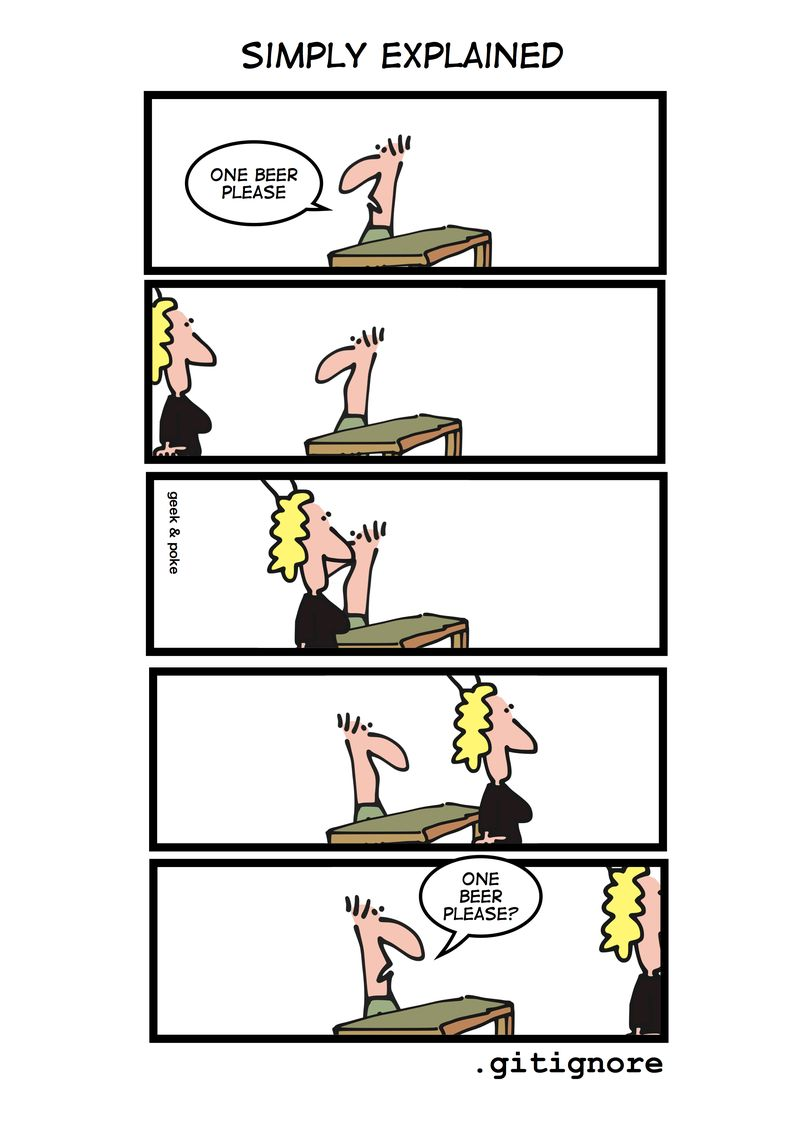
\includegraphics[angle=0,
                     width=0.6\textwidth]
                     {meinbild.jpg}
    \caption{Neulich in der Bar}
    \label{pic:inderbar}
\end{figure}
\end{lstlisting}

                  
\begin{figure}[htbp]
% Bild einfügen                
    \centering
\fbox{   
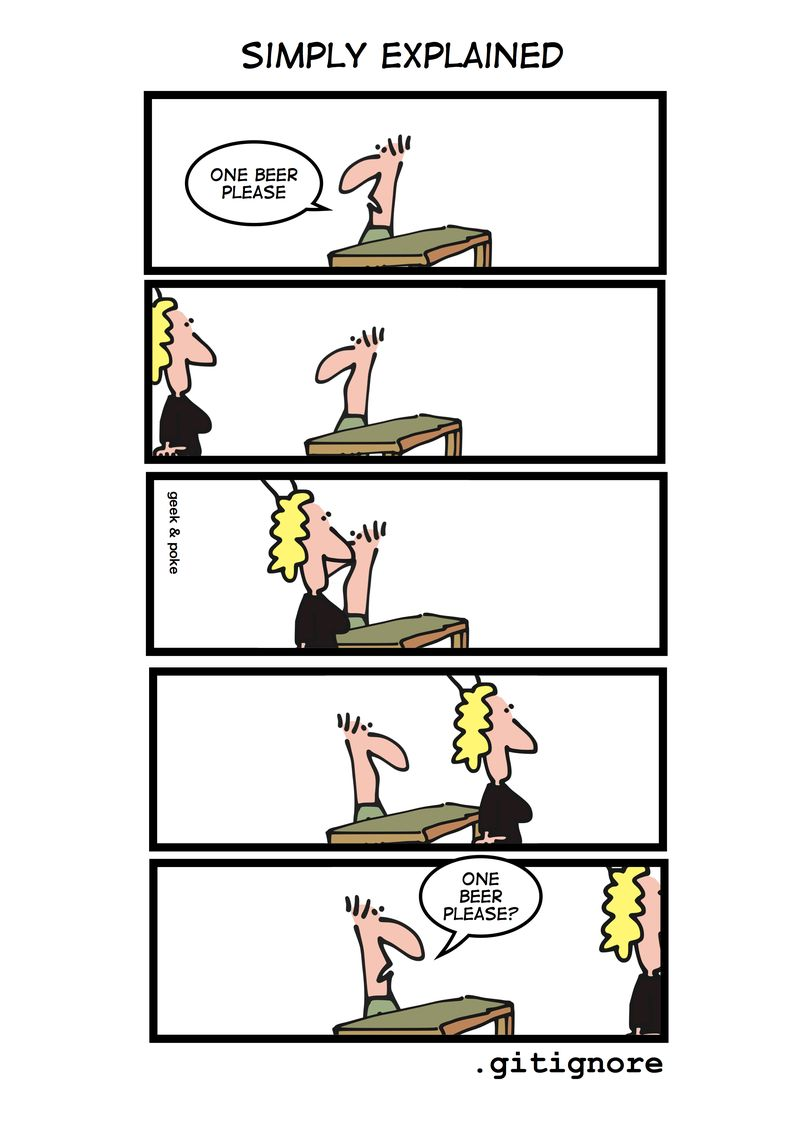
\includegraphics[angle=0,width=0.6\textwidth]{meinbild.jpg}}
    \caption{Neulich in der Bar}
    \label{pic:inderbar}
\end{figure}


\noindent
Zu dem Listing gibt es noch das eine oder anderen zu
erklären:

\begin{description}
    \item \lstinline|[htbp]| Beschreibt wie die Figur
positioniert           wird.
           Jeder der Buchstaben stellt einen Parameter dar.
           Mit der Reihenfolge htbp ergibt das die
           Anweisung; stelle mein Bild bitte hier hin (h
           für here) falls das nicht geht bitte das Bild
           nach oben schieben (t für top) falls das auch
           nicht geht dann eben nach unten (b für bottom)
           und falls das dann auch nicht gehen sollte, dann
           stells doch auf eine neue Seite (p für
           pagebreak).
    \item \lstinline|[angle=0]| Erlaubt das drehen des
Bildes
           (0-360 Grad). Hier mit 0 eingestellt.
    \item \lstinline|[width=0.6\textwidth]| Skaliert das
Bild. Hier
            zum 0.4-fachen der Textbreite. Zu
            beachten ist, dass           Textbreite nicht
            immer der breite des aktuellen          
            Absatzes entspricht. Beispielsweise bei Texten  
            mit mehreren Spalten beschreibt Textbreite die  
            Breite des Textes über die gesamte Seite. Möchte
            man die Bilder der Spalte (Kolonne) angepasst   
            haben so kann statt \lstinline|\textwidth| der  
            Parameter \lstinline|\columnwidth| verwendet    
            werden.
\end{description}



\section{Brief}

\begin{lstlisting}[caption=Allgemeine Settings,
                   label={lst:simplelist}]{Name}
\documentclass[11pt]{g-brief}
\usepackage[utf8]{inputenc}
\usepackage{ngerman}
\usepackage{enumerate}
\usepackage{eurosym}
\lochermarke
\faltmarken
\fenstermarken
\trennlinien                   
\end{lstlisting}

\begin{lstlisting}[caption=Angaben Absender,
                   label={lst:simplelist}]{Name}
% Angaben des Absenders
\Name                {Max Sendermann}
\Strasse             {Senderstrasse 99}
\Zusatz              {}
\RetourAdresse       {}
\Ort                 {6000 Luzern}
\Land                {Schweiz}

\Telefon             {+41/41 450 88 77}
\Telefax             {+41/41 450 88 78}
\Telex               {}
\HTTP                {www.sendermann.ch}
\EMail               {info@sendermann.ch}

\Bank                {Post-Finance}
\BLZ                 {}
\Konto               {40-123456-05}

\Unterschrift        {Max Sendermann}                  
\end{lstlisting}

\begin{lstlisting}[caption=Postvermerk und Empfaenger,
                   label={lst:simplelist}]{Name}
% Sendungsart/Postvermerk
\Postvermerk         {A-Post}

% Angaben des Empfängers
\Adresse             {Moritz Empfängermann\\
                      Empfangsstrasse 11\\
                      8600 Zürich}                  
\end{lstlisting}

\begin{lstlisting}[caption=Betreff und Datum,
                   label={lst:simplelist}]{Name}
% Betreff, Datum und Zeichen

\Betreff             {Empfangsbestätigung}

\Datum               {\today}
\IhrZeichen          {}
\IhrSchreiben        {}
\MeinZeichen         {}
\end{lstlisting}

\begin{lstlisting}[caption=Briefinhalt,
                   label={lst:simplelist}]{Name}
% Anrede & Gruss
\Anrede              {Sehr geehrter Herr Empfängermann,}
\Gruss               {Mit freundlichem Gruss}{1cm}

% Anhang/Anlagen
\Anlagen             {eBay-Kaufbestätigung\\
                      Einzahlungsschein}
\Verteiler           {}

% Briefinhalt
\begin{document}
\begin{g-brief}
Wie per Mail vereinbart, sende ich Ihnen hiermit die
Empfangsbestätigung des von Ihnen auf eBay erworbenen
Artikels. Die von eBay generierte Kaufbestätigung und der
quittierte Einzahlungsschein sind als Kopie hinterlegt zu
diesem Brief als Anlage.
\end{g-brief}
\end{document}

\endinput                 
\end{lstlisting}

\begin{figure}[htbp]
% Bild einfügen                
    \centering
\fbox{   
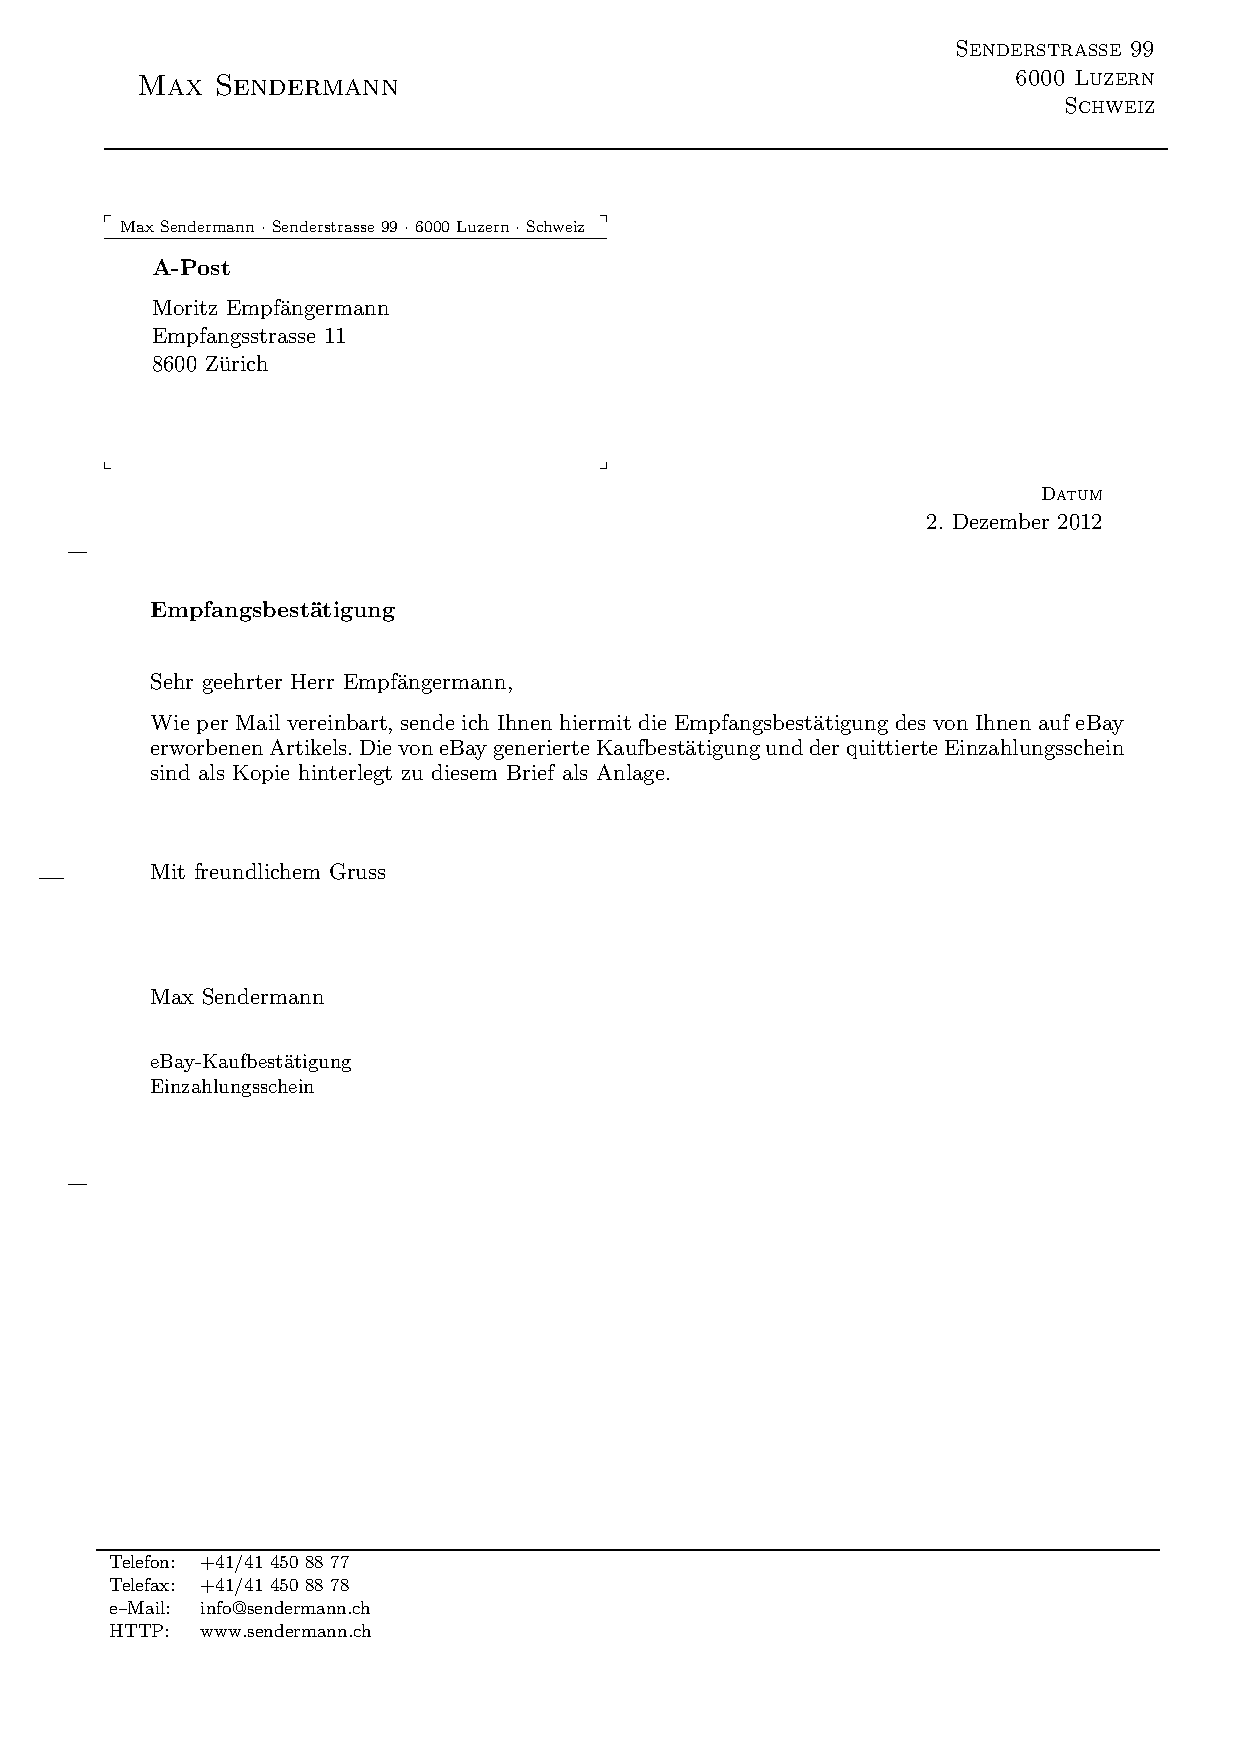
\includegraphics[width=1.0\textwidth]{briefm_muster.pdf} }
    \caption{Brief}
    \label{pic:inderbar}
\end{figure}
\section{Tabellen}

\indent
Tabellen in \LaTeX~zählen sicherlich zu den
Königsdisziplinen, denn meist ist man sich gewohnt sehr
viele Formatierungen zu benutzen (Ausrichtungen, Farben,
Einrückungen etc.). Will man von Anfang an ``komplexe''
Tabellen erstellen (von Hand) so fällt man leicht auf die
Nase oder tut sich schwer, da dies wirklich eine starke
Umgewöhnung ist.

Um das Prinzip einer Tabelle zu erläutern dient das
folgende Snippet.

\begin{center}
\begin{lstlisting}[caption=Einfache Tabelle]{easytable}
% Einfache Tabelle

\begin{tabular}{r l c}
Tag         & Haupttätigkeit        & Stunden \\
Montag      & Erholen vom Weekend   & 8 \\
Dienstag    & arbeiten              & 8 \\
Mittwoch    & arbeiten              & 8 \\
Donnerstag  & Kernel-Updates prüfen & 12 \\
Freitag     & weekend vorbereiten   & 4 \\
Samstag     & feiern                & 24 \\
Sonntag     & schlafen              & 24 \\
\end{tabular}
\end{lstlisting}
\end{center}

% Einfache Tabelle
\fbox{\parbox{0.9\columnwidth}{
\begin{tabular}{r l c}
Tag         & Haupttätigkeit        & Stunden \\
Montag      & Erholen vom Weekend   & 8 \\
Dienstag    & arbeiten              & 8 \\
Mittwoch    & arbeiten              & 8 \\
Donnerstag  & Kernel-Updates prüfen & 12 \\
Freitag     & weekend vorbereiten   & 4 \\
Samstag     & feiern                & 24 \\
Sonntag     & schlafen              & 24 \\
\end{tabular}
}}

\begin{description}
    \item \lstinline|[tabular]| ist eine Tabellenumgebung
die viele Parameter setzt (wie etwa Ausrichtung, Position
etc.).
    \item \lstinline|[{r l l}]| weist \lstinline|tabular|
an, dass eine Tabelle erzeugt werden soll mit drei Spalten
(entsprechend den drei Buchstaben \lstinline|r l l|) und
dass die 1. Spalte rechtsbündig ist (denn der erste
Buchstaben ist \lstinline|r| für right), die 2. soll
linksbündig sein (\lstinline|l| für left) und die 3. Spalte
soll zentriert werden (\lstinline|c| für center).
\end{description}

\noindent
Um Spalten und Zeilen mit Linien zu Trennen, so wie das oft
gewünscht ist bei Tabellen, kann ein \lstinline|\hline|
eingefügt werden um horizontale Linien zu erstellen und ein
\lstinline||| und Spalten voneinander zu trennen.

\begin{center}
\begin{lstlisting}[caption=Tabelle mit
Trennstrichen]{linetable}
% Einfache Tabelle mit Trennstrichen

\begin{tabular}{r | l | c}
Tag         & Haupttätigkeit        & Stunden \\
\hline
Montag      & Erholen vom Weekend   & 8 \\
Dienstag    & arbeiten              & 8 \\
Mittwoch    & arbeiten              & 8 \\
Donnerstag  & Kernel-Updates prüfen & 12 \\
Freitag     & weekend vorbereiten   & 4 \\
Samstag     & feiern                & 24 \\
Sonntag     & schlafen              & 24 \\
\end{tabular}
\end{lstlisting}
\end{center}

% Einfache Tabelle mit Trennstrichen
\fbox{\parbox{0.9\columnwidth}{
\begin{tabular}{r | l | c}
Tag         & Haupttätigkeit        & Stunden \\
\hline
Montag      & Erholen vom Weekend   & 8 \\
Dienstag    & arbeiten              & 8 \\
Mittwoch    & arbeiten              & 8 \\
Donnerstag  & Kernel-Updates prüfen & 12 \\
Freitag     & weekend vorbereiten   & 4 \\
Samstag     & feiern                & 24 \\
Sonntag     & schlafen              & 24 \\
\end{tabular}
}}\\\\

\noindent
Eine professionelle Tabelle beinhaltet aber nebst passenden
Ausrichtungen der Zellen auch eine allgemein passende Form.
So sollte eine gute Tabelle auch eine Indexierung haben.
Mein Vorschlag um gute Tabellen zu erstellen ist wie folgt.

\begin{center}
\begin{lstlisting}[caption=Bessere Tabelle]{goodtable}
% Bessere Tabelle

\begin{table}[htbp]
\fbox{\parbox{0.9\columnwidth}{
\begin{tabular}{| r | l | c |}
\hline
Tag         & Haupttätigkeit        & Stunden \\
\hline
Montag      & Erholen vom Weekend   & 8 \\
\hline
Dienstag    & arbeiten              & 8 \\
\hline
Mittwoch    & arbeiten              & 8 \\
\hline
Donnerstag  & Kernel-Updates prüfen & 12 \\
\hline
Freitag     & weekend vorbereiten   & 4 \\
\hline
Samstag     & feiern                & 24 \\
\hline
Sonntag     & schlafen              & 24 \\
\hline
\end{tabular} }} \newline\newline
\caption{Wochenüberblick}
\label{tab:wochenueberblick}
\end{table}
\end{lstlisting}
\end{center}


\begin{table}[htbp]
\centering
\fbox{\parbox{0.9\columnwidth}{
\begin{tabular}{| r | l | c |}
\hline
Tag         & Haupttätigkeit        & Stunden \\
\hline
Montag      & Erholen vom Weekend   & 8 \\
\hline
Dienstag    & arbeiten              & 8 \\
\hline
Mittwoch    & arbeiten              & 8 \\
\hline
Donnerstag  & Kernel-Updates prüfen & 12 \\
\hline
Freitag     & weekend vorbereiten   & 4 \\
\hline
Samstag     & feiern                & 24 \\
\hline
Sonntag     & schlafen              & 24 \\
\hline
\end{tabular} }} \newline\newline
\caption{Wochenüberblick}
\label{tab:wochenueberblick}
\end{table}

\noindent
Wird die Tabelle so erzeugt. so ist diese auch indexiert
und somit kann diese im Tabellenverzeichnis aufgelistet
werden. Dies ist oft verlangt bei grösseren Arbeiten.

\section{Literaturverzeichnis}

\noindent
Literaturverzeichnisse sind eine sehr wichtige Komponente
in vielen Arbeiten und man sollte diese verwenden.

Ein solches in \LaTeX~zu erstellen ist relativ einfach. Man
erstellt ein separates File welches die Quellen beinhaltet.
Dieses wird dann Zusammen mit dem Tool \BibTeX~genutzt zur
Erzeugung der Verzeichnisse. 

Viele Verlagseiten und auch z.B. die Wikipedia bietet einen automatischen
Export für \BibTeX~Einträge. Hier ein Beispiel zum Wikipedia-Artikel zu \LaTeX. \cite{wiki:latex}

\begin{center}
\begin{lstlisting}[caption=BibTeX Export aus Wikipedia]{wikibib}
@misc{ wiki:latex,
   author = "Wikipedia",
   title  = "LaTeX --- Wikipedia{,} Die freie Enzyklopädie",
   year   = "2012",
   url    = "http://de.wikipedia.org/w/index.
             php?title=LaTeX&oldid=110063618",
   note   = "[Online; Stand 2. Dezember 2012]"
 }
\end{lstlisting}
\end{center}

\noindent
Möchte man diese Quelle in seinem Dokument zitieren so gibt es je nach Style 
des Zitierens ein anderes Kommando. Bei der in diesem Werk empfohlenem APA Style
genügt es einfach \lstinline|\cite{wiki:latex}| zu schreiben.

\begin{description}
    \item \lstinline|[@misc]| weist \BibTeX~an, dass es sich bei dieser Quelle
    vom typ misc (Abkürzung von miscellaneous, also ``diverses'') handelt.
    Falls man ein Buch zitier möchte so gibt man stattdessen \lstinline|@book| 
    ein etc.
    \item \lstinline|[wiki:latex]| ist das Makro für diese Quelle. D.h. man 
    schreibt im Dokument eben dieses Makro um auf diese Quelle zu referenzieren.
    \item \lstinline|["Wikipedia"]| Statt die Gänsefüsschem zu schreiben kann man
    auch einfach geschweifte Klammern verwenden \lstinline|{Wikipedia}|.
    Hier ist noch nützlich zu wissen, dass doppelte Geschweifte Klammern  die 
    Inhalte innerhalb der Geschweiften Klammern nicht verändert in ihrer 
    Gross- Kleinschreibung. Dies gilt aber nicht immer. Oft geht es auch ohne.
\end{description}

\noindent 
Hier folgt nun ein Beispiel von einem Bib File mit verschiedenen Quellen.

\begin{center}
\begin{lstlisting}[caption=BibTeX Datei mit verschiedenen Quellen]{masterbib}
@misc{ wiki:latex,
   author = "Wikipedia",
   title  = "{LaTeX --- Wikipedia{,} Die freie Enzyklopädie}",
   year   = "2012",
   url    = "http://de.wikipedia.org/w/index.
             php?title=LaTeX&oldid=110063618",
   note   = "[Online; Stand 2. Dezember 2012]"
 }
 
@Book{kompakt_latex,
  author     = "Reinhard Wonneberger",
  title      = "Kompaktfuehrer LaTe{X}",
  address    = "Bonn",
  year       = "1988",
  descriptor = "LaTeX, TeX",
}

@Book{lamport_latex,
  author    = "Leslie Lamport",
  title     = "{{\LaTeX}}",
  publisher = "Cyfronet",
  address   = "Krak{\'o}w",
  pages     = "x + 202",
  year      = "1991",
  bibdate   = "Wed Jun 22 18:19:42 MDT 2005",
  bibsource = "alpha.bn.org.pl:210/INNOPAC;
               http://www.math.utah.edu/pub/
               tex/bib/texbook3.bib",
  note      =  "Polish translation of ``{\LaTeX}: 
                A Document Preparation System'', 
                1986, by Piotr Wyrostek.",
  acknowledgement = "Nelson H. F. Beebe, University 
         of Utah, Department
         of Mathematics, 110 LCB, 155 S 1400 E RM 
         233, Salt Lake City, UT 84112-0090, USA, 
         Tel: +1 801 581 5254, FAX: +1
         801 581 4148, e-mail: \path|beebe@math.utah.edu|,
         \path|beebe@acm.org|, \path|beebe@computer.org|
         (Internet), URL:
         \path|http://www.math.utah.edu/~beebe/|",
  language =    "Polish",
  subject  = "LATEX; podr{\k{e}}cznik",
}

\end{lstlisting}
\end{center}

\noindent
Die im Dokument zitierten Werke werden bei der Compilation\footnote{Immer 
zuerst \BibTeX ausführen und dann \LaTeX, da \LaTeX~die Ergebnisse aus \BibTeX~
einbindet. Es ist eine typische \LaTeX~Gewohnheit die Compilationen jeweils 
mehrfach durchzuführen, da verschachtelungen oft nicht rekursiv auf einmal 
ausgeführt werden können.} in das Literaturverzeichnis eingefügt.

Möchte man alle Quellen aus dem \BibTeX~File aufgelistet haben, unabhängig 
davon ob diese zitiert wurden so kann man \lstinline|\nocite{*}| verwenden.




% Abbildungsverzeichnis einfügen
\listoffigures

% Tabellenverzeichnis einfügen
\listoftables

% Listing-Verzeichnis
\lstlistoflistings

% Abkürzungsverzeichnis einfügen
% >>> Die Liste der Abkürzungen ist in einem separaten File
\include{meine_abkuerzungen}			

% Literaturverzeichnis einfügen
\nocite{*}								% alle Quellen auflisten
\bibliography{literatur}				    % Bibliographie wählen (BibTex Datei)
\bibliographystyle{apacite}				% Zitationsstyl wählen (hier nach APA-Norm)

% Ende des Dokumenteninhaltes
\end{document}
